\documentclass[10pt,a4paper]{article}
\usepackage[utf8]{inputenc}
\usepackage[german]{babel}
\usepackage{mathrsfs}
\usepackage{amsmath}
\usepackage{amsfonts}
\usepackage{amssymb}
\usepackage{amsthm}
\usepackage[left=2cm,right=2cm,top=2cm,bottom=2cm]{geometry}
\usepackage{graphicx}
\usepackage{listings}

\begin{document}

\section{Aufgabe 14}

\subsection{Teil a}

\subsection{Teil b}

\section{Aufgabe 15}

\subsection{Teil 1}

\subsection{Teil 2}

\subsection{Teil 3}

\subsection{Teil 4}

\section{Aufgabe 16}

\subsection{Teil 1}

\begin{lstlisting}
figure;
X = (1:0.01:9);
x = [0, 0, 2, 1, 0, 2, 2, 0, 2];
y = [0, 2, 2, 2.5, 2, 0, 2, 0, 0];
plot(x, y, 'c', spline((1:9), x, X), spline((1:9), y, X), 'r');
axis([-0.5, 2.5, -0.5, 3]);
\end{lstlisting}

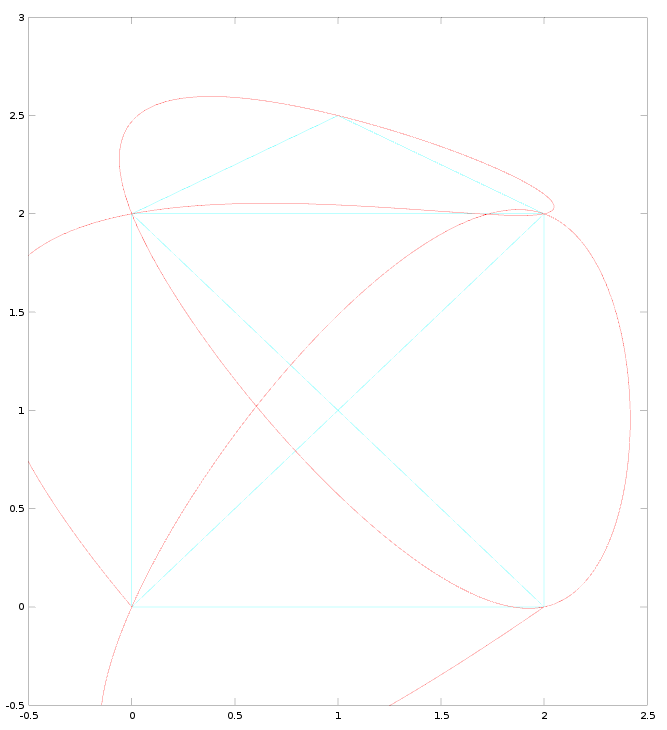
\includegraphics[width=300pt]{4_16_1.png}

\subsection{Teil 2}

\begin{lstlisting}
figure;
X = (1:0.01:17);
x = [0, 0, 0, 1, 2, 1.5, 1, 0.5, 0, 1, 2, 2, 2, 1, 0, 1, 2];
y = [0, 1, 2, 2, 2, 2.25, 2.5, 2.25, 2, 1, 0, 1, 2, 1, 0, 0, 0];
plot(x, y, 'c', spline((1:17), x, X), spline((1:17), y, X), 'r');
axis([-0.5, 2.5, -0.5, 3]);
\end{lstlisting}

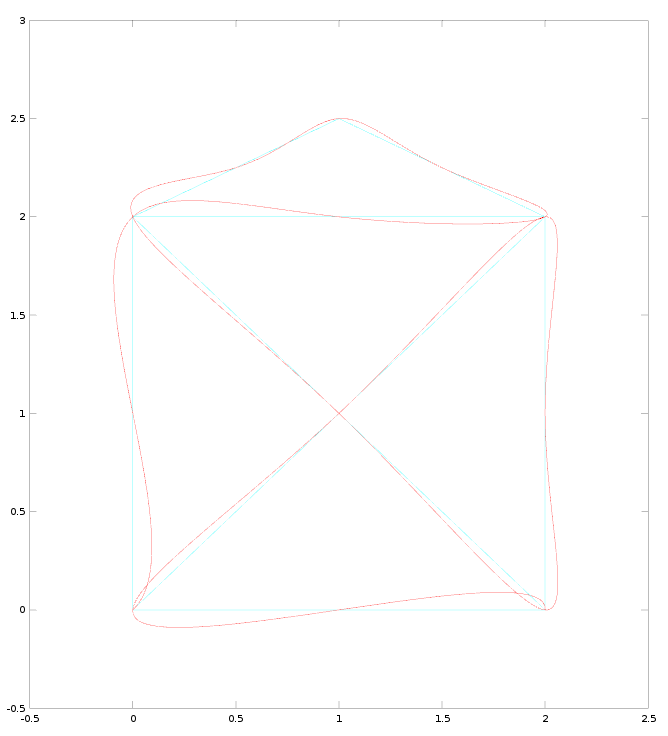
\includegraphics[width=300pt]{4_16_2.png}

\end{document}